%\documentclass[english,10pt]{beamer}
\documentclass[english,handout]{beamer}






 
%\usepackage{mathptmx}
%\renewcommand{\sfdefault}{lmss}
\usepackage[T1]{fontenc}
%\usepackage[latin9]{inputenc}
\usepackage[utf8]{inputenc}

\synctex=-1

\usefonttheme{professionalfonts}

%\setbeamertemplate{navigation symbols}{}
%\setbeamertemplate{caption}[numbered]


\useinnertheme{rectangles}
%http://tex.stackexchange.com/questions/11168/change-bullet-style-formatting-in-beamer

 \AtBeginDocument{
  \addtolength\abovedisplayskip{-0.4\baselineskip}%
  \addtolength\belowdisplayskip{-0.4\baselineskip}%
}%change the space between text lines and the math formula


\usepackage{pifont}
%Postscript ZipfDingbats font
%the command \ding{number}, will print the specified symbol

\usepackage{fontawesome}
%icon package
\DeclareFontFamily{U}{FontAwesomeOne}{}
\DeclareFontShape{U}{FontAwesomeOne}{m}{n}{<-> FontAwesome--fontawesomeone}{}
\DeclareRobustCommand\FAone{\fontencoding{U}\fontfamily{FontAwesomeOne}\fontseries{m}\fontshape{n}\selectfont}
\DeclareFontFamily{U}{FontAwesomeTwo}{}
\DeclareFontShape{U}{FontAwesomeTwo}{m}{n}{<-> FontAwesome--fontawesometwo}{}
\DeclareRobustCommand\FAtwo{\fontencoding{U}\fontfamily{FontAwesomeTwo}\fontseries{m}\fontshape{n}\selectfont}
\DeclareFontFamily{U}{FontAwesomeThree}{}
\DeclareFontShape{U}{FontAwesomeThree}{m}{n}{<-> FontAwesome--fontawesomethree}{}
\DeclareRobustCommand\FAthree{\fontencoding{U}\fontfamily{FontAwesomeThree}\fontseries{m}\fontshape{n}\selectfont}

%ftp://ftp.dante.de/tex-archive/fonts/fontawesome/doc/fontawesome.pdf
%http://tug.ctan.org/info/symbols/comprehensive/symbols-a4.pdf


\usepackage{amsmath,amssymb,amsfonts,bm,mathrsfs,mathtools}

\usepackage{tikzsymbols}
%\usepackage[tikz]{bclogo}



\usepackage{perpage}
\MakePerPage{footnote} %reset for each page
%\renewcommand{\thefootnote}{\fnsymbol{footnote}} %use symbol, limit less than 9 symbols



%%%% HIGHTLIGHT  and annotation &=%%%%%%%%
\usepackage{color,xcolor}
 \usepackage{todonotes}

\usepackage[normalem]{ulem}

\usepackage[many]{tcolorbox}

\tcbset{fonttitle=\scriptsize}
\tcbset{highlight math style={enhanced,
  colframe=red!40!black,colback=yellow!20!white,arc=2pt,boxrule=.2pt,
  }}
  \newtcbox{\otherbox}[1][]{nobeforeafter,math upper,tcbox raise base,
enhanced,frame hidden,boxrule=0pt,interior style={top color=green!10!white,
bottom color=green!10!white,middle color=green!50!yellow},
fuzzy halo=1pt with green,#1}
%%\tcbhighmath{math here}
%% \otherbox{math here}



%%%%% HIGHLIGHT %%%%%%
\newcommand{\hb}[1]{{\color{blue}{#1}}}
%\noindent\rule{\textwidth}{.5pt}

%:
\usepackage{soul}

\newcommand\hcancel[2][black]{\setbox0=\hbox{$#2$}%
\rlap{\raisebox{.45\ht0}{\textcolor{#1}{\rule{\wd0}{1pt}}}}#2}
%cross to delete

\newcommand{\mcb}[2]{\colorbox{#1}{$\displaystyle #2$}}
%highlight math

\newcommand{\hlfancy}[2]{\sethlcolor{#1}\hl{#2}}
%specified color , for\hl

\newcommand\myhl{\bgroup\markoverwith
  {\textcolor{yellow}{\rule[-.5ex]{2pt}{2.5ex}}}\ULon}



\mode<presentation>{ \usetheme{boxes} }

%write Matlab code
\usepackage{listings}
 \definecolor{dkgreen}{rgb}{0,0.6,0}
\definecolor{gray}{rgb}{0.5,0.5,0.5}
\definecolor{mauve}{rgb}{0.58,0,0.82}
\lstset{frame=tb,
  language=Matlab,
  aboveskip=3mm,
  belowskip=3mm,
  showstringspaces=false,
  columns=flexible,
  basicstyle={\small\ttfamily},
  numbers=none,
  numberstyle=\tiny\color{gray},
  keywordstyle=\color{blue},
  commentstyle=\color{dkgreen},
  stringstyle=\color{mauve},
  breaklines=true,
  breakatwhitespace=true
  tabsize=3
}

\usepackage[lastexercise]{exercise}

\newtheorem{ex}{Exercise}
\newtheorem{property}{Property}
\newtheorem{ag}{Algorithm}
\newtheorem{remark}{Remark}
\newtheorem{den}{definition}
\newtheorem{assumption}{Assumption}


\usepackage[nosolutionfiles]{answers}
\Newassociation{sol}{Solution}{ans}



\usepackage{empheq}
\usepackage{comment}
%\usepackage{lscape}
\usepackage{multirow}
\usepackage{url,hyperref}

\hypersetup{
 %   bookmarks=true,         % show bookmarks bar?
    unicode=false,          % non-Latin characters in Acrobat's bookmarks
    pdftoolbar=true,        % show Acrobat's toolbar?
    pdfmenubar=true,        % show Acrobat's menu?
    pdffitwindow=false,     % window fit to page when opened
    pdfstartview={FitH},    % fits the width of the page to the window
    pdftitle={My title},    % title
    pdfauthor={Author},     % author
    pdfsubject={Subject},   % subject of the document
    pdfcreator={Creator},   % creator of the document
    pdfproducer={Producer}, % producer of the document
    pdfkeywords={keyword1} {key2} {key3}, % list of keywords
    pdfnewwindow=true,      % links in new window
    colorlinks=true,       % false: boxed links; true: colored links
    linkcolor=red,          % color of internal links (change box color with linkbordercolor)
    citecolor=green,        % color of links to bibliography
    filecolor=magenta,      % color of file links
    urlcolor=cyan           % color of external links
}


\usepackage{subfigure,epsfig,graphicx,graphics}

\DeclareGraphicsRule{.tif}{png}{.png}{`convert #1 `dirname #1`/`basename #1 .tif`.png}
   \DeclareGraphicsExtensions{.pdf}




\newcommand{\hw}{ {\underline{\tt Homework }} }
\newcommand{\hws}{ {\underline{\tt Homework$\star$}} }
\newcommand{\optional}{ {\it optional} }

\newcommand{\MATLAB}{ \texttt{MATLAB}}
\newcommand{\python}{ \texttt{python}}
\newcommand{\Rlang}{ \texttt{R}}
\newcommand{\SAS}{ \texttt{SAS}}
\newcommand{\MC}{Markov Chain}


\newcommand{\tm}{transition matrix}
\newcommand{\rv}{random variable}
\newcommand{\spl} {supervised learning }
 

\newcommand{\dis}{\underline{\tt discussion}: }
\newcommand{\pri}{\underline{\tt principle}: }




\newcommand{\bq}{\scalebox{6}{\textbf{?} }}
\newcommand{\sq}{\scalebox{2}{\textbf{?} }}
\newcommand{\ck} {  {\scalebox{0.8} {\Interval}   } }

\newcommand{\eps}{\varepsilon}
\newcommand{\To}{\longrightarrow}

% 
\newcommand{\Dcal}{\mathtt{D}}
\newcommand{\Hcal}{\mathcal{H}}
\newcommand{\Ecal}{\mathcal{E}}
\newcommand{\Xcal}{\mathcal{X}}
\newcommand{\Ycal}{\mathcal{Y}}
\newcommand{\Zcal}{\mathcal{Z}}

%%Calculus 

\renewcommand{\d}{\ensuremath{\mathrm{d}}}
\newcommand{\dt}{ \ensuremath{\mathrm{d} t } }
\newcommand{\dx}{ \ensuremath{\mathrm{d} x} }
\newcommand{\dy}{ \ensuremath{\mathrm{d} y } }

%indicator function
\newcommand{\indf}{ \ensuremath{\mathbf{1} } }



%probability
\newcommand{\p}{ \mathbb{P}}
\newcommand{\prob}{{\Pr}}
\newcommand{\PP}{\mbox{PP}}%Poisson process
%condition prob
\newcommand{\cPr}[2]{{\Pr\left(#1\mid #2\right)}}

\newcommand{\FF}{{\mathbb{F}}}

\newcommand{\e}{ \operatorname{\mathbb E}}
\newcommand{\Var}{\operatorname{\mathbb{V} }}
\newcommand{\var}{\operatorname{\text{Var} }}
\newcommand{\MSE}{\operatorname{\text{MSE} }}

\newcommand{\Std}{\operatorname{std}}
\newcommand{\Cov}{\operatorname{cov}}

%Matrix  %mathbf
\newcommand{\Pb}{{\mathbf{P}}}
\newcommand{\Qb}{{\mathbf{Q}}}
\newcommand{\Mb}{{\mathbf{M}}}
\newcommand{\cb}{\mathbf{c}}
\newcommand{\bb}{{\mathbf{b}}}

\newcommand{\Tb}{\mathbf{T}}

\newcommand{\Wb}{\mathbf{W}}
\newcommand{\wb}{\mathbf{w}}
\newcommand{\Xb}{\mathbf{X}}

\newcommand{\xb}{\mathbf{x}}

\newcommand{\Wtn}{\mathbb{W}}
\newcommand{\btn}{\mathbf{b}}



\newcommand{\eye}{{\mathbf{I}}}
%identity matrix
\newcommand{\onem}{{\mathbb{1}}}
\newcommand{\idor}{\mathbf{1}}
\newcommand{\ii}{\mathbf{i}}
%imaginary symbol

\usepackage{tikz}

%State number
\newcommand{\snum}[1]{ \raisebox{.5pt}{\textcircled{\raisebox{-.9pt} {#1}}}}

 \usetikzlibrary{arrows}
\usetikzlibrary{shapes}

%\newcommand{\snum}[1]{%
 % \tikz[baseline=(char.base)]\node[anchor=south west, draw,rectangle, rounded corners, inner sep=1.4pt, minimum size=5mm,
   % text height=1.3mm](char){\ensuremath{#1}} ;}

\newcommand*\circled[1]{\tikz[baseline=(char.base)]{
            \node[shape=circle,draw,inner sep=.4pt] (char) {#1};}}


%real number
\newcommand{\Real}{{\mathbb{R}}}
%integer
\newcommand{\ZZ}{\mathbb{Z}}
%positive integer
\newcommand{\NN}{\mathbb{N}}



\newcommand{\inpd}[2]{\left\langle #1, #2 \right\rangle}
\newcommand{\abs}[1]{\left\vert#1\right\vert}
\newcommand{\norm}[1]{\left\|#1\right\|}
\newcommand{\wt}[1]{{\widetilde{#1}}}
\newcommand{\set}[1]{\left\{#1\right\}}
\newcommand{\partiald}[2]{  \frac{\partial #1 }{\partial #2}}



\newcommand{\ie}{{\it{i.e.}}}



\newcommand{\transpose}{\textsf{T}} % or, \intercal
\newcommand{\diag}{\textsf{diag}}
\newcommand{\tr}{{\textsf{T}}}
\newcommand{\rt}{{\textbf{r}}}

\DeclareMathOperator{\trace}{Trace}


\newcommand{\argmin}{ \operatornamewithlimits{argmin} }
\newcommand{\argmax}{ \operatornamewithlimits{argmax} }




\def\biz{\begin{itemize} }
\def\bizp{\begin{itemize}[<+->] }
\def\eiz{\end{itemize}}


\def\bfm{\begin{frame}}
\def\efm{\end{frame}}

\def\bena{\begin{enumerate}[<+-| alert@+>]}
\def\ben{\begin{enumerate}}
\def\een{\end{enumerate}}


\def\bbk{\begin{block} }
\def\ebk{\end{block}}






\makeatletter
%%%%%%%%%%%%%%%%%%%%%%%%%%%%%% Textclass specific LaTeX commands.
 % this default might be overridden by plain title style

%%%%%%%%%%%%%%%%%%%%%%%%%%%%%% User specified LaTeX commands.
%\usetheme{Warsaw}
\usetheme{Boadilla}
% or ...



%\setbeamertemplate{footline}[text line]{} % makes the footer EMPTY
%\setbeamertemplate{footline}[page number]{} % makes the footer EMPTY

%\usecolortheme{orchid} %not use is better 

\setbeamertemplate{footline}[text line]{%
  \parbox{\linewidth}{\vspace*{-2pt}Xiang Zhou\hfill CityU\hfill \insertpagenumber}}
%\setbeamertemplate{navigation symbols}{}

%\setbeamercovered{transparent}
% or whatever (possibly just delete it)


%\usepackage{babel}
\makeatother



 %
%\addtobeamertemplate{frametitle}{}{%
%\begin{tikzpicture}[remember picture,overlay]
%\node[anchor=south east,yshift=2pt] at (current page.south east) {
\includegraphics[height=0.6cm]{CityU_Logo_Basic_Signature.eps}};
%\end{tikzpicture}}
%

\beamerdefaultoverlayspecification{<+->}
%the presentation acts as though a \pause command has been inserted between every two bullets, without the actual need to write \pause after each item.



\title{Classification: LDA and  Logistic Regression}
\author{
\includegraphics[height=1.1cm,width=2.2cm]{../CityU_Logo_Basic_Signature.eps}
\\ $\ $ \\
Xiang Zhou  \\ $\ $ \\
}
\institute[]{  School of Data Science 
\\
 Department of Mathematics
\\
City University of Hong Kong
\\
~~
\\
\textup{  }
}

\date[]{}



\begin{document}
 
 


\maketitle
 


 
%%%-----------------------------------------------------------------
\frame{
~~{\huge \hb{Review of Bayes Classifier}}
}
    
%%%-----------------------------------------------------------------
\frame{{  0-1 loss}
We use 0-1 loss to evaluate the performance of classifiers.
 
The  zero-one  ($0$-$1$) loss function h
for the labelled class $y$ and the predicted class $\hat{y}$
is defined  
\footnote{In logistic regression, it is $h$, the pdf, not the
class label $\hat{y}$,
that shows in the loss function}, 

\begin{equation}\label{01loss}
\tcbhighmath
{\ell_{01}(y,\hat{y})=\idor(y \neq \hat{y})}\triangleq \begin{cases}
1 & \mbox{if }  y \neq \hat{y} \\
0   & \mbox{if }  y = \hat{y}  
\end{cases}
\end{equation}
where the misclassifications are charged by a single positive unit.
 
\begin{remark}[other equivalent forms]
If the binary outcome is encoded as $\set{-1,+1}$, 
then $\ell_{01}(y,\hat{y})= 1-\mbox{heaviside} (y  \hat{y})
= (1-\mbox{sign}( y\hat{y}))/2$
where $\mbox{heaviside}(t) = \begin{cases}
1  &  ~~\mbox{if} ~~  t\geq 0 
\\
0  &  ~~\mbox{if} ~~ t< 0
\end{cases}
$ and $\mbox{sign}(t)=\begin{cases}
1  &  ~~\mbox{if} ~~  t\geq 0 
\\
-1  &  ~~\mbox{if} ~~ t< 0
\end{cases}$.
So 0-1 loss is equivalent to 
$-\mbox{heaviside} (y  \hat{y})
$ and $-\mbox{sign}(y  \hat{y})$.
\end{remark}


}


%%%-----------------------------------------------------------------
\frame{
  For any classifier  \myhl{$G: \mathcal{X}\to \set{1,\ldots, K}$}, its 0-1 loss 
overall  test error rate 
is \begin{equation}\label{01error}
\begin{split}
\e_{X,Y} \left [ \ell_{01}(Y, G(X)) \right]& = \e_{X}  \left (  \sum_{k=1}^K \ell_{01}( k , G(X)) 
 \times \p ( Y=k \vert X)
 \right)
 \\
 &=1-
  \e_{X} \Big[    \p ( Y= G(X) \vert X)
\Big]~\because \ell_{01} \mbox{ is 0-1 loss}
\end{split}
\end{equation}
So,   
\[
\inf_{G} \e_{X,Y} \left [ \ell_{01}(Y, G(X)) \right]
\]
is equivalent to 
\[
{\sup_{G } \e_{X} \Big[    \p ( Y= G(X) \vert X)
\Big]
}
\]
which has the following  {optimal solution} defined point-wisely for $x$:
\[
G^*(x) = \argmax_{k\in\set{1,\ldots,K}}  \p ( Y= k \vert X=x)
\]
}

%%%-----------------------------------------------------------------
\frame{

\begin{definition}[{\bf Bayes classifier}]
\[ 
\tcbhighmath
{
G_{bayes}^*(x) = \argmax_{k\in\set{1,\ldots,K}}  h_k(x) 
} \]
where \[h_k(x) := \p ( Y= k \vert X=x)]\] 
 \end{definition}
\bigskip
 {\rule{\paperwidth}{0.2pt}}

 
\begin{definition}[{\bf Gibbs classifier}]
Given an input $x$, the predicted class is 
a random sample from $\set{1,\ldots, K}$ according to the 
prob mass fun $
\set{h_k(x), 1\leq k\leq K}
$
\end{definition}
 This also works well. 

 }
 
 
%%%-----------------------------------------------------------------
\frame{{\faLightbulbO~ Bayes classifier is optimal
for misclassification error}

~{  Recall for regression, the conditional probability $f(x)=\e (Y\vert X=x)$
minimizes the squared error loss $\e [ \abs{Y-f(X)}^2]$
 and the conditional median $f(x)=\mbox{median}(Y\vert X=x)$
 minimizes the $L_1$ error loss $\e \abs{Y-f(X)}$.
For classification, we have the analogy for the Bayes classifier.}



\begin{theorem}
Bayes classifier minimizes the expected $0$-$1$ loss.
\end{theorem}
 
  
The    0-1 loss  of Bayes classifier 
is called  {\bf Bayes error rate}:
\[ 1 - \e_X \left[ \max_{k}\p( Y=k\vert X)  \right]
=1-\e_X \left[ \max_{k} h_k(X)  \right].\]

 
 }





%%%-----------------------------------------------------------------
\frame{{Bayes Theorem for Bayes Classifier}
 \biz
 
\item The  {\bf Bayes theorem }
is to view this as the 
{\it posterior} distribution
of $Y$ with the given observation $X=x$:   
\begin{equation}
\label{eqn:BayesC}
\begin{split}
h_k(x)&=\p(Y = k|X = x) 
\\
&= \frac{\color{red}{\p(X = x | Y=k) } {\color{blue} {\p(Y=k)} }  }
{
 \p(X=x)
}
\\ 
& =: \boxed{
 \frac{ {\color{red}{\rho_k(x)} }  { \color{blue}{\pi_k } } } { \sum_{l=1}^K \rho_l(x) \pi_l } 
 }
\end{split}
\end{equation}
\item 
${\color{red}{\rho_k(x)} }$:
{\bf the class-conditional  pdf of $X$} in class $Y=k$;
\item 
${ \color{blue}{\pi_k } } $:
the (prior) distribution of the class $Y$ ;
\item 
For any given $x$, 
the conditional pmf of  $Y$ is 
\[
\tcbhighmath
{
h_k(x) \propto \rho_k(x)\pi_k.
}\]

\item 
One might estimate   $\rho_k(x)$ ( ``density estimation'') and  $\pi_k$ ( the fraction of training examples belong to class $k$ ) directly from the data. 
  
 
  \eiz
}

%%%-----------------------------------------------------------------
\frame{
{ Bayesian  classifier}
\biz

\item {\bf Bayesian  classifier}
assigns each observation to the most likely class, given its predictor value $x$,
i.e.,  classifies into the maximal posterior  prob.
\begin{equation} \label{BC}
G^*(x) =  
\argmax_{1\leq k\leq K} \p ( Y=k \vert X=x)
=\argmax_{1\leq k\leq K}   ~ [f_k (x)\pi_k]
\end{equation} 

This is called \underline{Brute Force MAP ({\it maximum a posterior}) Learner} in Computer Science .

\item {\it Bayes decision boundary} is the decision boundary determined by this 
 Bayes  classifier.
 

\item The joint distribution of $(X,Y)$ is $\p(X=x,Y=y)=\sum_{k=1}^K \rho_k (x)\pi_k$.
Then this  model is the typical mixture models: 
convex combination of 
$K$ distributions of $f_k$:
connection to missing data problem, EM algorithm.
 
  \eiz
}



%%%-----------------------------------------------------------------
\frame{%%%-----------------------------------------------------------------
\frametitle{mixed Gaussian:   $\rho_k \sim \mathcal{N}(\mu_k,\sigma^2_k)$}
Recall the posterior distribution in   \eqref{eqn:BayesC}
$ \p(Y = k|X = x)  = 
 \frac{ {\color{red}{\rho_k(x)} }  { \color{blue}{\pi_k } } } { \sum_{l=1}^K \rho_l(x) \pi_l }
 $
 where $\rho_k(x) \triangleq\p(X = x | Y=k)$ is the distribution of $X$ conditioned on $Y=k$.
  Bayes classifier maximize this over $k$.
\begin{ex}
{\bf Assume} that $X\in \Real^1$ and  $\rho_k \sim \mathcal{N}(\mu_k,\sigma^2_k), ~1\leq k\leq K$.
   
Then the Bayes classifier corresponds to the maximizer $k^*$ of the following 
  discriminant function 
\begin{equation}\label{eqn:LDA2} 
\delta_k(x) =-\frac{x^2}{2\sigma_k^2} +x \cdot \frac{\mu_k}{\sigma_k^2} - \frac{\mu_k^2}{2\sigma_k^2} + \log \pi_k.\end{equation}
When $K=2$, find the point corresponding  to the   Bayes decision boundary.
\end{ex}
   } 





 
 %%%-----------------------------------------------------------------
\frame{{{\bf Naive} Bayesian Classifier
 } 
 If $\mathcal{X}$ has a dimensionality $d \gg 1$, then the class-conditional pdf $\rho_k(x)$ 
 is a high dim fun of $x$.
  The  ``naive ''  idea in Naive Bayesian classifier is to {\bf ASSUME} that 
 each component is independent !
 
 
\[
\rho_k(x)=\rho_k(x_1,\ldots,x_d) = \prod_{j=1}^d \rho_{kj}(x_j)
\] 
 

 BENEFIT:  decompose a high dim problem (intractable in density estimation)  to low dim problems.
 \par
 JUSTIFICATION:  works surprisingly well in practice for {\bf certain problems}.     
 
 \begin{quote}
 ``Along with decision trees, neural networks, k-nearest neighbours,
the Naive Bayes Classifier is one of the most practical
learning methods.''
 \end{quote}
 }
 
 %%%-----------------------------------------------------------------
\frame{{Bayes learning: Bayesian Belief Network}
 Bayesian Belief Network assumes the $k$ class-conditional pdf 
 dependency in the form of a network representing 
the conditional information  (causal knowledge).  
 \[ \rho_k(x_1,\cdots, x_d)= \p( X=(x_1,\cdots, x_d)\vert Y=k)\]
  
   
 }
 
 %%%-----------------------------------------------------------------
\frame{
{Linear/Quadratic Discriminant Analysis (LDA/QDA)}

Recall the mixed Gaussian model \eqref{eqn:LDA2}
above but in $d$ dimension,


Assuming $X | ~Y=k \sim \mathcal{N}_d( \mu_k, \Sigma_k)$,
the $d$-dim Gaussian distribution,  then
$$
\delta_k(X)=\log(\pi_k) - (1/2) \log |\Sigma_k| -  (1/2) (X-\mu_k)^T \Sigma^{-1}_k (X-\mu_k).
$$
Classify $x$ to class $k$ with the largest $\delta_k(x)$.

\begin{itemize}
\item $\hat \pi_k = n_k /n$: the ratio of samples belonging to class $k$ in totally $n$ 
population;
\item $\mu_k$ is estimated by the centroid in each class $k$
\item $\Sigma_k$ is estimated by sample covariance matrix 
with each class $k$
\end{itemize}


\biz
\item
{\bf Assuming} that all $\Sigma_k$ are equal
(estimated by pooled sample variance matrix $\hat{\Sigma}$), 
we can reduce $\delta_k$ to a {\bf linear} function in $x$ ;
 \item
The {\bf QDA} method  use  the original  {\bf quadratic} function 
$\delta_k$,
but QDA need estimate the in-class variance $\sigma_k$
or the covariance  matrix $\hat{\Sigma}_k$ in high dim $\Real^d$, $d>1$.
This requires more data than the LDA for better estimation.
\item 
The decision boundary of QDA is (quadratically) curved. 
\eiz
}
 

%%%------------------------------------------
%%%-----------------------------------------------------------------
\frame{

\begin{ex}
Ex. 4.2. [ESL]
\end{ex}


\begin{ex}
In LDA, consider the eigen-decompositon  of the sample covariance matrix $\hat{\Sigma}$ and derive the reduced rank LDA.
\end{ex}
}
%%%------------------------------------------



 

%%%-----------------------------------------------------------------
\frame{ {   \faWrench ~  $k$-NN (nearest neighboring) methods}
%%%-----------------------------------------------------------------
\framesubtitle{a non-parametric approach to regression and classification}
  $k$-NN   method
  \footnote{{\tiny \faWarning}~   $k$
  is the number of points in constructing a neighbourhood.
  Not to be confused  with index previously used for the labels of $K$ classes. }: directly estimate the conditional expectation/probability
from the data $\Dcal=\set{(x_i,y_i): 1\leq i\leq n}$.
\par
\biz
\item 
%Read Section 3.5 in [ISLR].
\[ 
\mbox{For regression:
} \e(Y\vert X=x) \approx \mbox{AVE} (y_i \vert  x_i \in N_k(x)):=\frac{1}{k}
\sum_{i:  x\in N_k(x) }  y_i .\]
 \item
 \[\mbox{For classification: } \p(Y=class\vert X=x) \approx \frac{1}{ k} \sum_{i\in N_k(x)} \idor( y_i =class)\]
where $N_k(x)$ is the collection of 
 $k$  points in $\set{x_i}$   {\it closest}
  to $x$.
 \eiz

}

   



%%%-----------------------------------------------------------------
\frame{
{Logistic, LDA, QDA,  k-NN ?
 %Alchemy or Chemistry ? 
 }
%%%-----------------------------------------------------------------
\framesubtitle{ model selection -- to be addressed later}
\begin{quote}[p154, [ISL]]
``When the true decision boundaries are linear, then the LDA and logistic regression approaches will tend to perform well. When the boundaries are moderately non-linear, QDA may give better results. Finally, for much more complicated decision boundaries, a non-parametric approach such as KNN \footnote{with correct choice of $k$ such as by the cross-validation} can be superior. ''
\end{quote}
 

}


\section{Logistic
Regression}

%%%-----------------------------------------------------------------
\frame{{Logistic
Regression  }

\biz
\item Today, the logistic
regression model is one of the most widely used binary models in the analysis of
categorical data where $\Ycal=\set{1,\ldots,K}$.
\item Logistic regression,  an extension of the linear regression for classification,
is  based on modeling the {\it odds} of an outcome:
\[
\p(Y=k\vert X=x),
\]
{in contrast to} the outcome  $Y=k$ itself.

\item Before that, Fisher proposed {\it linear discriminant analysis} ({\bf LDA}) in 1936.
There are other methods based on the use of
some discriminant function, which 
may not be
$\p(Y=k\vert X=x)$.


\eiz
We focus on the following four questions which   we shall always follow for any machine learning problems
\ben
\item How to represent  the ``odds'' ?
\item How to model the the cost/loss functions ?
\item How to minimize the cost function?
\item How to evaluate the performance of the trained model ?  
\een
}


 %%%-----------------------------------------------------------------
\frame{{Logistic regression model for binary classification}
Now $\Ycal=\set{0,1}$.
Recall that in Bayes classifier, we introduced a function
$h(x)$ as the  
{\bf conditional probability} of 
$y=1$ for a given input $x$:
\[ h(x)=\p(Y=1 \vert X=x),~~ 1-h(x)=\p(Y=0  \vert X=x)\]

 
\biz
\item {  Assume} that  the logarithm of this probability,
as a function of $x$, 
 is  a \underline{linear} function:
  $ \log h(x;\theta )=f(x, \theta)=\theta \cdot x$, we 
 would have $h=e^{\theta\cdot x}$ which is always positive but has no upper bounds.
\item The modification is to use the ``0'' class probability 
(i.e. $1-h$) as a {\it reference value.}
Then the logistic regression model is  to assume that  \[
 \log h(x; \theta)  - \log (1-h(x; \theta)) = f(x;\theta)
\]
or 
\[
 h = \frac{1}{1+ e^{-f}}, ~~
 1-h = \frac{e^{-f}}{1+e^{-f}}
\]
Now, $f$ can be any $\Real$-valued continuous function  on $\mathcal{X}$.
You can propose any hypothesis space ($\subset \mathcal{X}$) you want
to search the best $f$ in this space. 
 \eiz
}

%%%-----------------------------------------------------------------
\frame{
 
\begin{definition}
The {\bf logit } function: $(0,1)\to \Real^1$  is 
\[ h\to z=\log \frac{h}{1-h}=: \mbox{logit}(h) \]
The inverse of logit function  is the {\bf sigmoid(logistic)}  function:  $\Real^1 \to (0,1)$
\[
z\to h  = \otherbox{ \sigma(z):=\frac{1}{1+ e^{-z}} }  \]
\end{definition}
\begin{center}
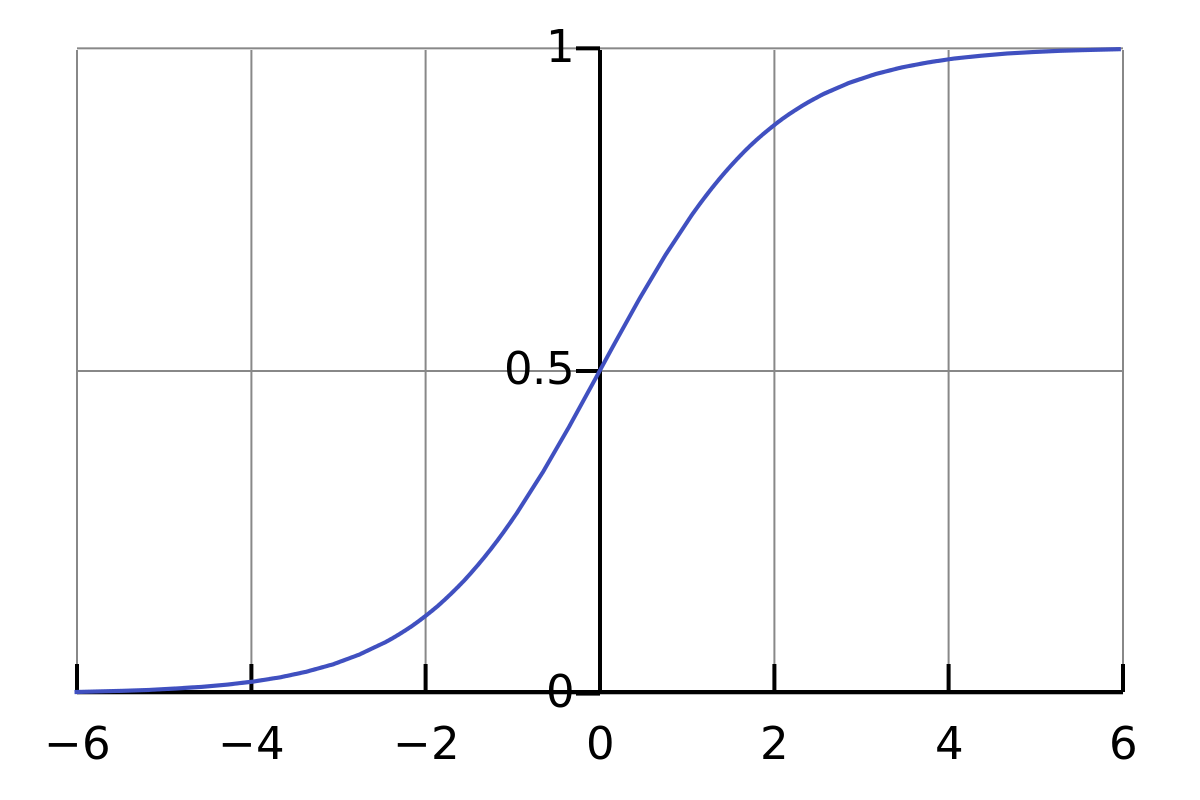
\includegraphics[scale=0.15]{sigmoid.png}
\end{center}
 }
 
 
 
 %%%-----------------------------------------------------------------
\frame {
 {activation function family}
 Why $\sigma$ this form  ? 
 \biz
 \item What kind of {\it activation} function mapping $\Real^1$ onto $(0,1)$?
 
\biz
\item   Heaviside  function $\sigma(x)=I_{\set{x>0}}$;
\item   capped linear function  $\sigma(x) = \max\set{\min(k x+c,1), 0}$  with   $k>0$, $c\in\Real$;
\item  $\sigma(x) = \frac{1}{\pi}\arctan (x)+\frac12$
\item  $\sigma(x) =\frac{1}{\sqrt{2\pi}} \int_{-\infty}^x e^{-x^2}dx$ ......
\eiz

\item  The considerations of  choosing the feature variable and 
the activation  function:

\biz
\item     simple  
\item    computational concerns in minimizing the loss
\item     Inverse function 
\item     some certain stat/prob. interpretation ( {\it log-odds} by  G. A. Barnard,1949 )  

\eiz

  
 \eiz
 
 }
 
 
 %%%-----------------------------------------------------------------
\frame{{Sigmoid logistic  function}
\biz
\item 
The logistic function was invented for the purpose of
describing the population growth (\href{https://papers.tinbergen.nl/02119.pdf}{history}).
Logistic map: $x_{n+1}=rx_n (1-x_{n})$.
  Logistic function  was given its name by a Belgian mathematician,
P.F. Verhulst (1838).
So, the logistic function is used in areas far beyond the classification.
\item The logistic function is an offset and scaled {\bf hyperbolic tangent function}:
 $\sigma(x)=\frac12 + \frac12 \tanh(z)$ because $\tanh(z)=\frac{e^z-e^{-z}}{e^z+e^{-z}}$.
\item  
$\sigma(x)$ is smooth and symmetric in the sense 
$$\sigma(x)+\sigma(-x)=1$$
\eiz

 }
 
 
 %%%-----------------------------------------------------------------
\frame
 {
 
 \begin{ex}
Show that the sigmoid function satisfies  the logistic equation
\[
 {\sigma'(z) =\sigma(z)(1-\sigma(z))}
\]
and show that if $h(x;\theta)=\sigma(z(\theta,x))$
for a general bi-variate function $z(\cdot,\cdot)$ of $\theta$ and $x$, then 
the gradient 
$\nabla_\theta h(x;\theta)=\sigma'(z)\nabla_\theta z $,
and the Hessian matrix
$
\nabla^2_\theta h(x;\theta) = \sigma''(z) \nabla_\theta z \nabla_\theta z^\tr 
+\sigma'(z) \nabla^2_\theta z
$ 
\end{ex}


\begin{ex}[softplus function]
Show that the derivative of the so called
{\bf softplus} function 
\[
\mbox{softplus}(x) = \ln (1+e^x) 
\]
is 
the sigmoid function $\sigma(x)=1/(1+e^{-x})$.
Equivalent
$\int_{-\infty}^x \sigma(x')\d x' = \mbox{softplus}(x) $.
In addition, show that 
$$-\log ( \sigma(z)) = \mbox{softplus}(-z)
~~\mbox{and} ~ 
-\log (1- \sigma(z)) = \mbox{softplus}(z)$$
So, softplus function is connected to the 
negative log likelihood function.
\end{ex}
Softplus function is 
a smooth function close to 
the RELU: $\mbox{RELU}(x)= \max(0,x)$

\href{https://www.desmos.com/calculator/4ophg8wvju}
{visualization}
}




%%%-----------------------------------------------------------------
\frame{
{framework}

We now have a general framework for classification problem
by working on the log-odd, $z$: 
\[
\boxed{
x\in \mathcal{X}\xrightarrow{ \hb{f(x;\theta)} } z \in \Real^1 
\xrightarrow{\sigma(\cdot)} h\in (0,1)
\xrightarrow [ h>0.5]{ h<0.5}
 y\in \mathcal{Y}=\set{0,1}
 }
\]

The decision boundary   $\set{x: h(x)=0.5}$ 
becomes   the set where $z=f(x;\theta)=0$ since $\sigma(0)=0.5$

\biz
\item  $z=\hb{f(x)>0} \iff h(x)>0.5$: classifies $x$ as  ``1''.
\item  $z=\hb{f(x)<0} \iff h(x)<0.5$:  classifies $x$ as  ``0''.
\item $z=\hb{f(x)=0} $ gives the decision boundary. 
\eiz

In summary, the classifier given by $f$
 is  to assigne $ x$ to the class
 $=\mbox{heaviside}(f(x))   
 =\mbox{heaviside}(h(x)-0.5)$
 
 
{\rule{\paperwidth}{0.2pt}}


What remains is to select a model class (hypothesis space
$\Hcal$)
for representing 
\[ x\in \mathcal{X}\xrightarrow{ \hb{f(x;\theta)} } z \in \Real^1 
 \]
\biz
\item Linear function   $z= \beta \cdot x + \beta_0 \Longrightarrow$  \hb{logistic regression}
linear decision  boundary (hyperplane)
\item Quadratic function;
or  any possibility of nonlinear functions
(like for the regression problem) 
\eiz

}
 
  
 %%-------------------------------------------%%

%%%-----------------------------------------------------------------
\frame{
{ Logistic regression model for $K>2$ classes} 
%%%-----------------------------------------------------------------
\framesubtitle
{Softmax regression (multinomial logistic regression) }

Generalize to the $K$-class where the labels $y\in \set{1,\ldots,K}$ by assuming 
that the conditional prob. takes the form
\begin{equation}\label{hk}
   \p(Y=k \vert X=x) = h_k(x;\theta)  
 \end{equation}
But we have the constraint  
$$\sum_{k}h_k(x;\theta)=\sum_k \p (Y=k \vert X=x)) =1.$$ 
WLOG, we use the last one $h_K(x;\theta)$.
Define   $   z_k$,
the {\bf logit},  
\[
 z_k:= {\log h_k (x;\theta) - \log h_K (x;\theta),      ~~ k=1,2,\ldots, K-1.}
\]
Then $h_k = h_K e^{z_k}
$ and   $z_K=0$. The constraint $\sum_k h_k=1$ leads to 
$h_K =\left(\sum_{k=1}^{K} e^{z_k }\right)^{-1}$ and
\begin{equation}
\label{eqn:hk}
\boxed{h_k (x;\theta) = \frac{e^{z_k}}{  \sum_{k=1}^{K} e^{z_k}}},    ~~k=1,2,\ldots K
\end{equation}

}


%%%--------------------------------------------------------------

%%%-----------------------------------------------------------------
\frame{{Softmax function}
\begin{definition}
 The {\bf softmax} function is the following nonlinear mapping $\Real^K \to  (0,1)^K$:  
 $$z=(z_1,\ldots,z_K) \mapsto h=(h_1,\ldots, h_K)=\mathtt{softmax}(z) $$ where
 \[
\tcbhighmath
{h_k = \frac{e^{z_k}}{\mathcal{Z}}, ~~\mbox{where} 
~~\mathcal{Z}:=\sum_{i=1}^K e^{z_i}
}
 \]
 i.e., $\log h_k = z_k - c$ where   $c$  is a constant such that 
 $\sum_{k=}^K h_k=1$.
\end{definition}
\begin{remark}
The name ``softmax''
comes from the fact
$\lim_{\delta \to 0}\mbox{softmax}(z/\delta) = (0,\ldots,0,1,0,\ldots,0)$ where the position of $1$ entry
corresponds to 
 $\argmax_k \set{z_k}$ .
\end{remark}

}
 
 
 %%%--------------------------------------------------------------

 %%%-----------------------------------------------------------------
\frame{
 
 It takes a vector of arbitrary real-valued scores  and squashes 
 the vector to a 
 new vector  with values between $0$ and $1$  and 
 with  zero sum. 
 
 \bigskip
\begin{ex}
\biz
\item 
If $z_1<z_2$, then $h_1<h_2$. So $h$ keeps the order of $z$ (and magnifies the difference among the values $\set{z_k}$)
\item
$\mathtt{softmax}(z+c)=\mathtt{softmax}(z)$ for any scalar $c$.
If choose $c=-\max\set{z_1,\ldots,z_K}$, then every elements in the vector $z+c$ is not positive.
The calculation of  $\mathtt{softmax}(z+c)$ is more stable than that directly on $\mathtt{softmax}(z)$.
($\exp(1000)$ gives you {\tt NaN}  on computers.)
\item When  $z_k=\theta_k \cdot x$, show that 
the shift $\theta  \to \theta  - c$ does not change the value of $h(x;\theta)$.
So  the  softmax regression's $K$ parameters are redundant.
In learning $\theta$,  we can simply set $\theta_K=0$
or adding the linear constraint $\sum \theta_k =0$.
\eiz
\end{ex}
}


%%%-------------------------------------------------------
%%%-----------------------------------------------------------------
\frame
{
{Linear model assumption  for $z_k$ }
\biz
\item 
With the aid of softmax, the representation 
of the function $\set{h_k(x)}$ becomes the representation of 
$\Real^K$-value functions ${z_k(x)}=f_k(x;\theta)$.

\item 
The softmax (logistic) regression assume the linear form 
$
z_k = f_k(x;\theta_k)=\theta_k \cdot x,
$
with $K$ parameters $\theta_k\in \Real^d$
\footnote{
Effectively, $K-1$ parameters,  since $z_K=0$.}.
For convenience, we still
 use ${  \theta}=\set{\theta_1,\ldots, \theta_K}$ to denote all the parameters of our model .
\item Like in nonlinear regression,
all same techniques can be applied
here to represent the function $x\to z_k$. 
(sparse, kernel, spline ,..... )
 \item
Recently, the DNN (deep neural network)
models the function $x\to z_k$ by neural network.
The result is a huge success.



 \eiz
 
 }
 
 %%%-----------------------------------------------------------------
\frame{
 {Decision rule of softmax regression}
 
\[
\boxed{
x\in \mathcal{X}\xrightarrow[k=1,\ldots,K]{ \hb{f_k(x;\theta)} } z_k \in \Real^1 
\xrightarrow{\mathtt{softmax}} h_k\in (0,1)
\xrightarrow [y=k^*]{ \max_k h_k(x)}
 y\in \mathcal{Y}=\set{0,1}
 }
\]


 $h(x;\theta)=\mathtt{softmax}(z)$ i.e.,
 $h_k (x;\theta) = \frac{e^{z_k}}{  \sum_{k=1}^{K} e^{z_k}}, k=1,2,\ldots K$ and  $z_k =f_k(x;\theta)= \theta_k \cdot x$.
Then for an input $x$,
we assign it to the class which is 
\[ \begin{split}
k^*(x) =&\argmax_{1\leq k\leq K} h_k(x;\theta)=\argmax_k e^{z_k}\\
=&\argmax_k z_k = \argmax_k f_k (x)
\\=&\argmax_k (\theta_k \cdot x)
\end{split} \]
The last step shows that it is a linear classifier
since $z_k$ is linear in $x$. 



\bigskip
Exercise:  For example, $K=3$, and $d=2$, $\theta_1=(1,0), \theta_2=(1,1), \theta_3=(0,0)$.
draw the three domains where $x$ are classified as $1,2,3$, respectively.
}



%%%-----------------------------------------------------------------
\frame{
{How to choose loss function}
\biz
\item A criterion must be set to
define the loss function $\ell$
in order to find the optimal parameter $\theta$
in $h_k(x;\theta)$.
\item 
We first recall that the 0-1 loss 
is defined for the classification outcome:
$\Ycal \times \Ycal \to \set{0,1}$.

\item 
 The predicted class
$\hat{y}(x)=\argmax_k h_k(x;\theta) $,
then 
$\ell_{01} (y,\hat{y})= I(y=\argmax_k h_k(x;\theta))$
\item
The empirical risk from the data $\Dcal=\set{(x_i,y_i)}$ is 
\begin{align*}
 \sum_{i=1}^N  I(y_i =\argmax_k h_k(x_i;\theta)) 
=\sum_{k=1}^K  \sum_{(x_i, y_i=k)}
I(k =\argmax_{k'} h_{k'}(x_i;\theta)) 
\end{align*}
\item For the binary case where $\Ycal=\set{0,1}$,
with $h(x;\theta)=h_1(x;\theta)$,
\begin{align*}
 &\sum_{i=1}^N  I(y_i =\argmax_k h_k(x_i;\theta)) 
\\
= & \sum_{(x_i, y_i=1)}
I(h(x_i;\theta)>0.5 ) 
+\sum_{(x_i, y_i=0)}
(1-I(h(x_i;\theta)>0.5)).
\end{align*}
\eiz

}


%%%-----------------------------------------------------------------
\frame{
 
 \biz
 \item
The above 0-1 loss only used the sign of 
$h(x)-0.5$; the prob. meaning of 
$h(x) $ is not used.
In addition, the minimization for the above
empirical 0-1 loss is hard.
 \item
 The key difference of logistic regression
 from most  machine learning methods  based on linear
 separating hyperplane (SVM)
 is that logistic regression 
attempt to model and 
estimate $\p(Y=k| X=x)$ for each $k$
directly .
  
  \eiz
  
 \bigskip
 \underline{~ Two  Main Principles
 to Build Loss functions}

{\Large
\biz
\item[\faLightbulbO~] Statistical Learning Approach:
\biz
\item Maximize Likelihood 
\item  Bayesian  = Prior  $\times $ Likelihood 
\eiz
\item[\faLightbulbO~]  Information Theory Approach:
 Minimize the ``distance'' between prob. measures.
\eiz
}
 
  
}





%%%-----------------------------------------------------------------
\frame{
{ Loss  function  of 
logistic regression = 
negative log-likelihood }
\href{https://www.coursera.org/learn/machine-learning/lecture/1XG8G/cost-function}{coursera video}.
\biz
\item  In linear regression, the   squared  error  $l(y,\hat{y})=(y-\hat{y})^2$,
 has the interpretation of
negative log  likelihood for Gaussian-type residuals.
 The same idea of taking 
negative log  likelihood as the loss 
for classification is  as follows.
\item For a given data point $(x,y)$, in binary case, the probability 
$\p(Y=y\vert X=x) = h(x;\theta)$   if $y=1$
and $\p(Y=y \vert X=x) = 1-h(x;\theta)$ if $y=0$, which can be unified in one expression
for the likelihood function:
\[
\p(Y=y\vert X=x)=h^{y}   (1-h)^{1-y},
\]
Then the 
\hb{ negative log-likelihood}  is 
 \[-   y\log h  - (1-y) \log (1-h)
\]
which is will be defined as $\ell$.
 Thus, MLE is equivalent to minimizing $\ell$.
\eiz
}
 
 %%%-----------------------------------------------------------------
\frame{
 {Loss function for Binary classification}

\begin{definition}
The loss function for the binary logistic regression
is  the function  $(0,1)\times \set{0,1} \to \Real^+$
in the form 
\begin{equation}
\ell(h,y)= - y \log h  -(1-y) \log (1-h)=\begin{cases}
-\log  h  & \mbox{ if } y=1 \\
-\log  (1-h )   & \mbox{ if } y=0 \\
\end{cases}
\label{loss-log}
\end{equation}
\end{definition}
 Note that 
 this form of this loss function 
is unlike   the regression loss where
the two input argument are both 
$\Ycal$-valued.
 
 \begin{columns}
\begin{column}{0.5\textwidth}
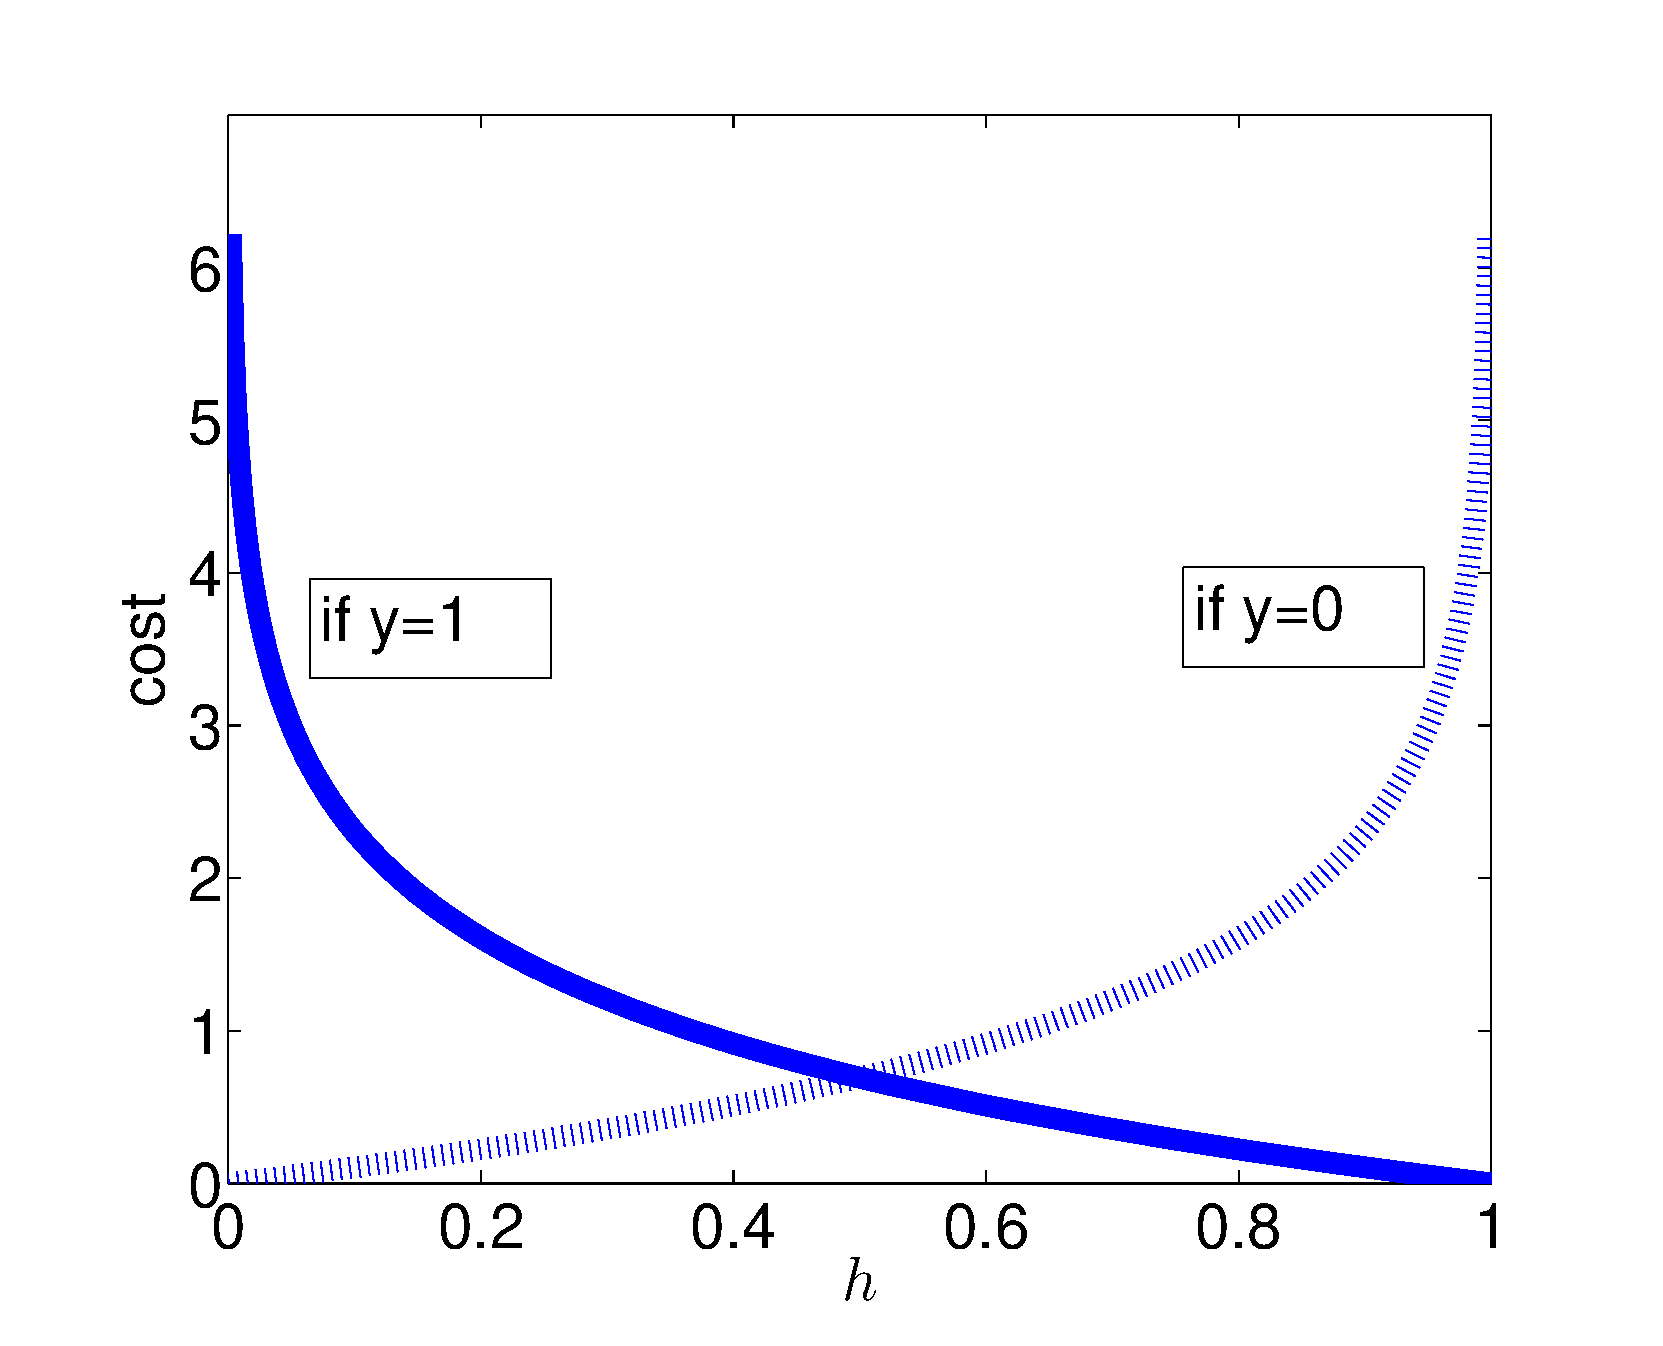
\includegraphics[width=0.8\textwidth,
height=0.6\textwidth]{logitcost.eps}
\end{column}
\begin{column}{0.5\textwidth}
\hw $\ell$ is convex in $h$.
\dis Why this cost fun makes sense from the viewpoint of minimizers at different values of $y$?
Derivative $\partial l /\partial h$
\end{column}
\end{columns}
 }
 
 %%%-----------------------------------------------------------------
\frame{
 Then the objective  function
 \footnote{sometimes, we drop the $\frac{1}{n}$ factor in $J$ since it does not affect the minimizers.}
 on the training dataset $\Dcal=\set{(X^{(i)}, Y^{(i)})}$ is the sum of loss 
 from all individual examples 
  \begin{equation}\label{eqn:losslogit}
 \begin{split}
 J(\theta) &= \frac{1}{n} \sum_{i=1}^n \ell ( h(X^{(i)};\theta), Y^{(i)})\\
 &= \frac{1}{n}\left(
  \sum_{ i:Y^{(i)} =1}  -\log h(X^{(i)};\theta)
 + \sum_{ i:Y^{(i)} =0}  -\log (1-h(X^{(i)};\theta) )
 \right)
 \\
 &= \frac{1}{n}\left(
  \sum_{ i:Y^{(i)} =1}
    \log  \Bigg(1+e^{ -f ( X^{(i)}; \theta) } \right)
    \\
    &
    \qquad \qquad 
 + \sum_{ i:Y^{(i)} =0} \log  \left(1+e^{ +f ( X^{(i)}; \theta) } \right)
 \Bigg).
  \end{split}
 \end{equation}
In logistic regression, 
$f(x;\theta)=\theta\cdot x$.

\begin{ex}
Show that $J$ is convex in $\theta$ 
for logistic regression.
\end{ex}

}




 \begin{frame}
 The following exercise shows that
 the binomial deviance loss
 is just the loss in logistic regression,
 written in terms of $f$ rather than of $h$.
 \begin{ex}
 Recall the relation that
 the odd $h=\sigma(z)$,
 $\sigma$ is the sigmoid function,
 and $z=f(x;\theta)$. Then  the logistic loss
 $\ell$ in \eqref{loss-log} can be written
 in terms of $f$,
 \footnote{  
 We here abused the use of $\ell$.
 The  definition domain of $\ell$ function here is $\Real\times \set{0,1}$,
 not $(0,1)\times \set{0,1}$.
  }
\begin{equation}
\ell(f,y)= \begin{cases}
-\log  h(x;\theta) = \log (1+e^{-f})
=\mbox{softplus}(-f) & \mbox{ if } y=1 \\
-\log  (1-h(x;\theta) ) = \log (1+e^f) 
=\mbox{softplus}(f)& \mbox{ if } y=0 \\
\end{cases}
\end{equation}
Change the  binary coding of $\Ycal$
to $\set{\pm 1}$
(i.e, ``$0$'' class is named as ``$-1$'' class now), then 
$\ell(f,y)$ has a convenient expression:
\begin{equation}
\otherbox{
\ell_{\text{bd}}(f,y):= \mbox{softplus} (-y f(x)), ~~
y\in\Ycal =\set{-1,1}, f : \Xcal \to \Real.
}
\end{equation}
which is 
\underline{ the product of $y$ and $f$.}
This loss
$\ell_{\text{bd}}(f,y)$ has the name
{\bf binomial deviance loss}, which 
arises from {\em deviance} statistics for binormal distribution.
\footnote{ 
The important concept of 
``deviance'' is not discussed further in this course
}
 \end{ex}
 \end{frame}

%%%-----------------------------------------------------------------
\frame{
In this page, we   use $\set{\pm 1}$-encoded $\Ycal$
and compare the 0-1 loss and the binomial 
deviance loss.
\biz
\item 
Note that the classifier with a given $f$
is equal to $\mbox{sign}(f(x))$.
Then the 0-1 loss can be rewritten as 
$\ell_{01}(y,f(x))=\mbox{heaviside}(-yf(x) )$.

\item Logistic regression: $\ell_{bd}(y,f(x))=\mbox{softplus} (-yf(x))$.

\item The third loss:
hinge loss  $\ell_{\mbox{hinge}}(y,f)=(1-yf)_+$
is used in support vector classifier  (to be discussed later)
\eiz

\begin{figure}[htbp]
\begin{center}
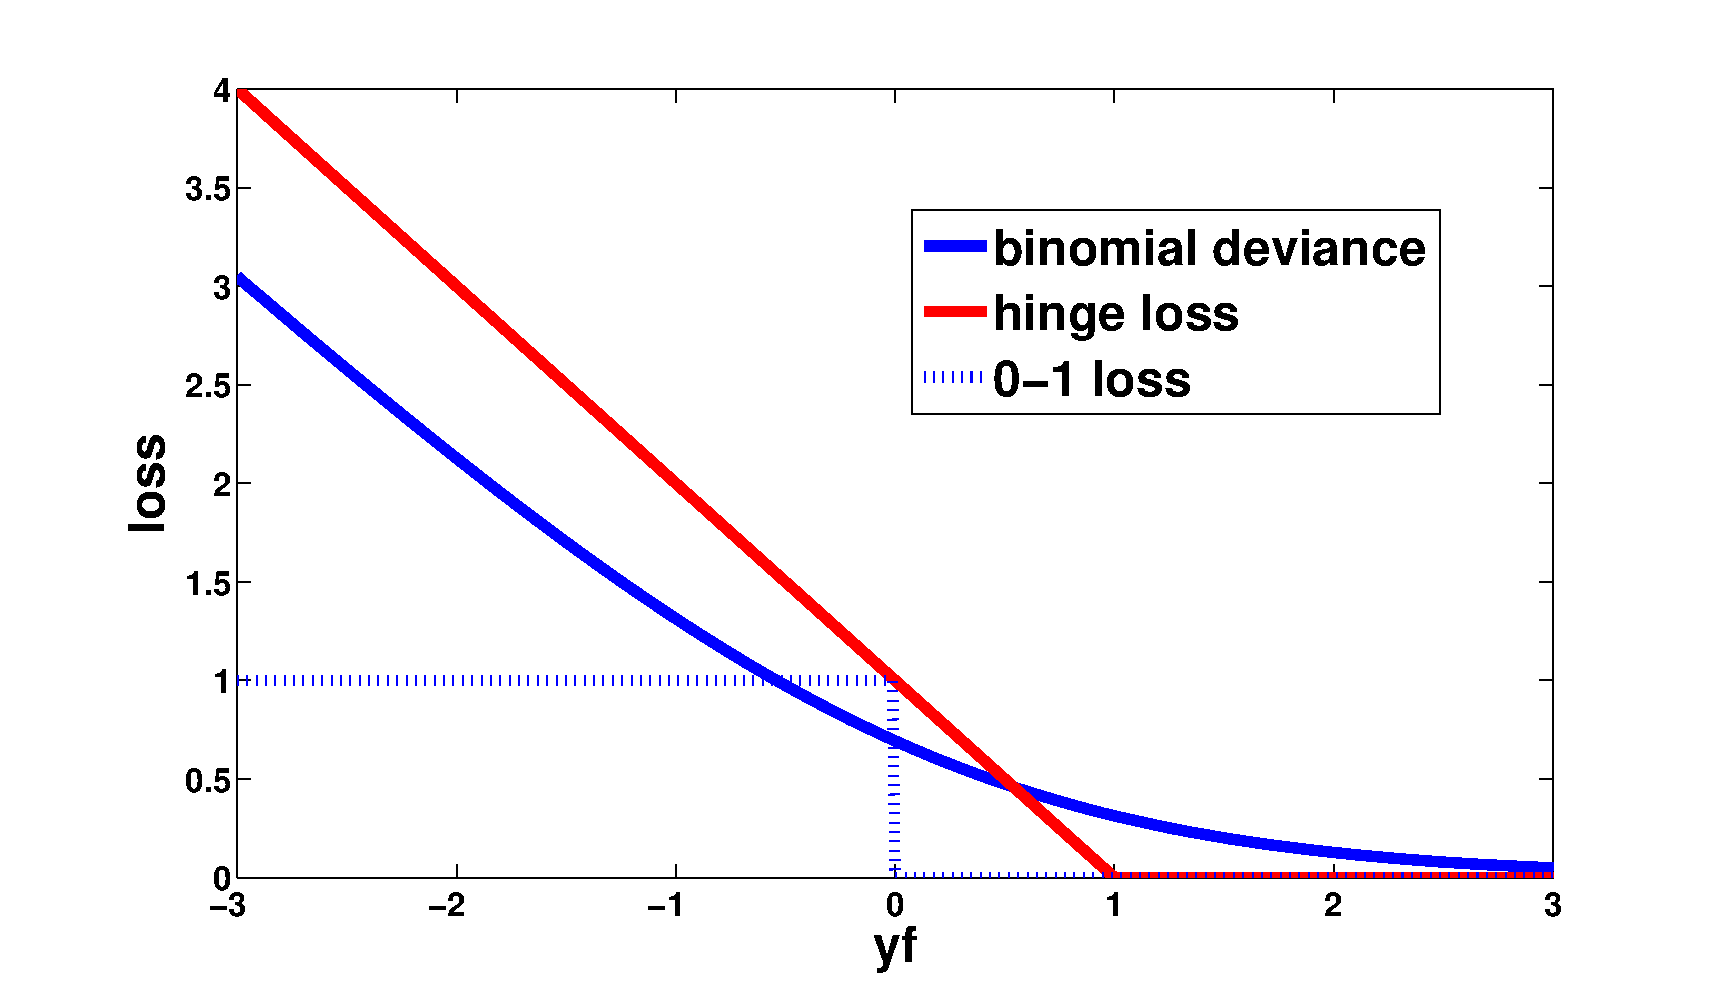
\includegraphics[width=0.6\textwidth]{lossclassification.eps}
  \end{center}
\end{figure}
}




%%%-----------------------------------------------------------------
\frame {

\begin{ex}
Recall in Topic 1,
we have $\Ecal$ defined as the expected loss
(the generalized error):
\[
\Ecal_{bd}( f) =  \e \ell_{bd}(Y,f(X))=\e_{X,Y} \left [
\mbox{softplus}( -Yf(X))
\right]
\]
Denote $\pi_\pm=\p(Y=\pm 1)$
the distribution of $Y$ 
and $\rho_\pm=p_{X | Y=\pm}(x)$,
the conditional distribution of $X$ given $Y$.
Solve the variational problem 
\[
\inf_f \Ecal_{bd}(f)
\]
Show that the optimal $f_*$
is  
\[\sigma(f_*(x))=\frac{\pi_+ \rho_+(x)}{
\pi_+\rho_+(x)+ \pi_- \rho_-(x)}
=\frac{\p(X=x, Y=+)}{p_X(x)}
=\p(Y=+\vert X=x)\] 
\end{ex}
This expression of  $f^*$
  is consistent to the fact that
$h(x)=\sigma(z)=\sigma(f(x))$.

}


%%%-----------------------------------------------------------------
\frame{{Loss function of $K$-classification }
\biz
\item 
 The  loss function
 as the negative log likelihood 
  for $K$-classification  on
an input-output   $(x,y)$ is
\begin{equation} \label{softmaxloss}
\ell({\bf h},y)  =\begin{cases}
-\log h_1(x;\theta)  & \mbox{ if }  y=1 \\
-\log h_2(x;\theta)  & \mbox{ if }  y=2 \\
\ldots  \ldots &\\
 -\log h_K(x;\theta)  & \mbox{ if }  y=K 
\end{cases}
=  \tcbhighmath
{ - \log h_y(x;\theta)
}
\end{equation}
where ${\bf h}=(h_1,\ldots h_K)=\mbox{softmax}
(z)$ with $z_k = f_k(x)=x\cdot \theta_k$.
 \item Then we have the objective function  
 \begin{equation}
 J(\theta):= \frac{1}{n}\sum_{i=1}^n  - \log h_{Y^{(i)}} (X^{(i)};\theta)=
 \frac{1}{n}
  \sum_{k=1}^K 
 \left( \sum_{
 \substack{  i\in \set{1,\ldots,n}
\\  Y^{(i)}=k }
}  -\log h_k(X^{(i)};\theta) \right)
 \end{equation}
 \item cross-entropy 
 \eiz
 
 }



 


 %%%-----------------------------------------------------------------
\frame{{Information Theory view:
   Loss function as the  cross-entropy } 

\begin{definition}

\biz
\item  The (Shannon) {\bf  entropy} of a prob. distribution $p$ is 
\[ H(p)=H(p,p)=-\e_{Y\sim p} [\log p(Y)]=-\sum_{y}  p(y) \log p(y). \]
\item 
 The {\bf cross-entropy} between  a  distribution $p$ and another  distribution $q$ is defined as:
\[ 
H(p,q)\triangleq-\sum_{y} p(y)\log q(y) = 
- \e_{Y\sim p} [\log q(Y)]
\]
\item  The {\bf Kullback-Leibler divergence}  is defined as
\[ \displaystyle D_{\mathrm {KL} }(p\|q) \triangleq -\sum _{x}p(x)\,\log {\frac {q(x)}{p(x)}}
=H(p,q)-H(p)
 \]
\eiz
\end{definition}
 }



 %%%-----------------------------------------------------------------
\frame{
\biz
\item
 $D_{\mathrm {KL} }(p\|q) $ is non-negative and is the measurement of how far from $q$  to $p$. Note that 
 $D_{\mathrm {KL} }(p\|q)\neq D_{\mathrm {KL} }(q\|p)$ in general. But 
 $D_{\mathrm {KL} }(p\|q)=0$ iff $p=q$.
 \item 
 For fixed $p$, minimizing $D_{\mathrm {KL} }(p\|q) $ over $q$ is equivalent to 
 minimizing $H(p,q)$.
\eiz
\bigskip
\hb
{How to choose $p$ and $q$ for classification problem ?
}
\biz
\item
In the above logistic regression for the $K$ classification, 
{\it given} $x$, $q$ is a Bernoulli distribution 
$q(k)=\p(Y=k\vert X=x)=h_k (x;\theta), 1\leq k\leq K$.
\item  
$p$ is from      one given sample 
$(x,y)\in \mathcal{X}\times \set{1,\ldots, K}$,
it  is the delta distribution 
({\bf one hot distribution}):
$ p(k) = 1 $ if $k=y$
and  $p(k) = 0 $ if $k\neq y$, i.e., $p(k)=\delta_{k,y}$
\item So,
$H(p,q)= -\sum_{k} p(k) \log q(k) = - \log h_y(x;\theta) $, which is identical to the loss \eqref{softmaxloss}

 \eiz
 This is why \eqref{softmaxloss}
called the {\bf cross-entropy  loss} or {\it log loss}.

 }
 
%  
%
%%%%-----------------------------------------------------------------
%\frame{
%\biz
%\item
%{Hellinger distance:}
%\[
%D_{H}( q,  p) = \left( \displaystyle \int_{\mathcal{X}}  \left(\sqrt{p(x)} -\sqrt{q(x)} \right)^2 \dx\right)^{1/2} 
%\]
%\item
%{Total variation distance:}
%\[
%D_{TV}(q, p) =   \sup_{A} \abs{\int_{A}p(x)-q(x)~\dx}
%\]
%\eiz
%\begin{ex}
%Le Cam's inequality 
%Prove that 
%\[D_{TV}(p,q)\leq D_{H}(p,q)\leq  (KL(q\| p))^{1/2}  \]
%\end{ex}
%
%}

%%%-----------------------------------------------------------------
\frame{{Numerical Optimization of Logistic Regression Models}
%%%-----------------------------------------------------------------
\framesubtitle{ gradient calculation }
Recall that ${\ell(h(x;\theta),y)= - y \log h(x;\theta)  -(1-y) \log (1-h(x;\theta))}$
and 
$h(x;\theta)=\sigma(z)$ where $z=f(x;\theta)=\theta\cdot x$.

\begin{equation*}
\begin{split}
\nabla_\theta \ell 
 &
 = -y/\sigma(z) \cdot \sigma'(z) \nabla_\theta z +  (1-y)/(1-\sigma(z))  \cdot \sigma'(z)  \nabla_\theta z
\\
 &
 = -y (1- \sigma(z)) \nabla_\theta z +  (1-y)    \sigma(z)  \nabla_\theta z
\\
& =  (\sigma(z)-y)\nabla_\theta z
= (h(x;\theta)-y) x
\end{split}
\end{equation*}

\begin{ex}
Show that the Hessian matrix 
of $\ell$ is  
$$\nabla_{\theta}^2  \ell  = (h(x;\theta)-y) \nabla^2_\theta z +
\sigma'(z) (\nabla_\theta z )
 (\nabla_\theta z )^\tr =  h(1-h)x   x^\tr .$$
Show that this matrix has the rank 1 and is  positive semi-definite.

\end{ex}


}

%%%-----------------------------------------------------------------
\frame{
\[ 
\begin{split}
J(\theta)&=  \sum_{i=1}^n \ell (h(x^{(i)}; \theta), y^{(i)})
\\
\nabla_\theta J &=\sum_{i=1}^n (h(x^{(i)};\theta)-y^{(i)}) x^{(i)}
= {\Xb} (\bf{\sigma( \bf z)-y}) \\
& \mbox{ where  } ~~ {\bf z} =  \Xb \theta
\end{split}
\]
Here, the matrix
$\Xb\triangleq [x^{(1)}, x^{(2)},\ldots, x^{(n)} ]\in \Real^{d\times n}$
whose $n$ {\it columns} corresponding to $n$ data points.
$\theta$ and ${\bf y}=(y^{(1)}, y^{(2)},\ldots, y^{(n)} )^\tr$ are column vectors.
$\sigma$ function acts on the vector in the    element-wise sense.

Then the gradient descent is 
\[ \theta^{new}= \theta^{old}+ {\mbox{learning rate}} \times \frac{1}{n}\sum_{i=1}^n (y^{(i)}-h(x^{(i)}; \theta^{old}) )x^{(i)}\]
Now consider the displacement $\Delta \theta:= \theta^{new}- \theta^{old}$
on the projection of $x^{(i)}$,
then $\Delta z^{(i)}=\Delta \theta \cdot x^{(i)} = \eta  (y^{(i)}-h(x^{(i)}; \theta^{old}) ) \norm{x^{(i)}}^2 $.
So, $y^{(i)}=1$ means $\Delta z^{(i)} >0$ and 
$y^{(i)}=0$ means $\Delta z^{(i)} <0$. Recall the decision boundary in $\mathcal{Z}$ space.
}
%

\end{document}


